%!TEX root = ../main.tex
An example of a node can be seen in figure \ref{fig:gps_node}.

\begin{figure}[!h]
\centering
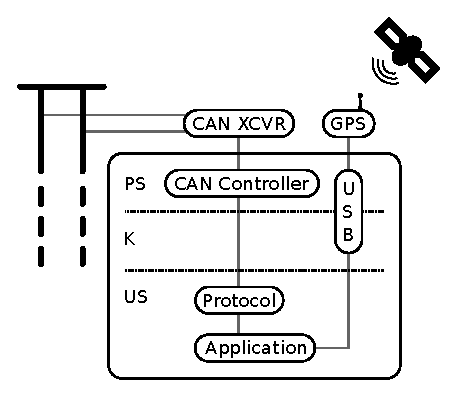
\includegraphics[width=0.5\textwidth]{graphics/analysis_gps.eps}
\caption{GPS node implemented on Zybo board.}
\label{fig:gps_node}
\end{figure}

This specific node has a GPS attached to it connected through a USB interface, but in general it could be any kind of data producing unit connected through any kind of interface.
From the analysis section is it clear that a node has the following responsibilities:

\begin{itemize}
\item Get data from associated sensor.
\item Pack data according to the specified protocol.
\item Construct CAN package
\item Send data using a CAN controller.
\item Get data from CAN network.
\item React to commands sent to it.
\end{itemize}

A node can be any kind of microcontroller, but this section will only address the case where a Zybo board is used as node microcontroller. 
The requirements state that it should be simple to add nodes to the system. 
To realize this the node software should be designed to be modular.
It should be easily identified what software and what interface a developer of a new node must adhere to.
The coming sections will explain the design of the node software that will provide the mentioned functionality using the design requirements.

The first section will explain the software running on the userspace in Linux, whereas the next section will address the use of the built in CAN controller.	

\subsection{Userspace Software}
To design modular software it needs to be analyzed which responsibilities are the same for all nodes and which are sensor specific.
The sensor specific tasks are found to be getting data from sensor and to pack data according to the specified protocol.
The remaining responsibilities are the same for all nodes in the system. 
A class diagram showing the designed software can be seen in figure \ref{fig:node_class_diagram}.
Left side is bla bla bla.

\begin{figure}[!h]
\centering
\missingfigure[figwidth=1\textwidth]{Class diagram}
\caption{Class diagram showing node software.}
\label{fig:node_class_diagram}
\end{figure}


\subsection{CAN Controller Software}
\mikkel{Catalins stuff should be here?}